\section{Excluding two further bases in a phase ball}
\label{sec:exclusion}

We now give a local exclusion procedure for a certified Hadamard phase
ball.  Its conclusion concerns every exact Hadamard in that ball,
including its boundary. Theorem~\ref{execute:finite-theorem} combines
these local conclusions with the exhaustive cover and the execution checks.

Two further bases would consist of two groups of six vectors, each vector
unbiased to the first two bases. Within either group the vectors are
pairwise orthogonal; across the groups every pair is unbiased. We first
cover all possible individual vectors by small closed balls in their
phase coordinates. We will show that the twelve vectors must have
distinct covering-ball labels. Necessary pair tests then give two graphs
on these labels: an edge is retained whenever the tests do not rule out
orthogonality or unbiasedness, respectively. The two bases would require
two disjoint orthogonality six-cliques with all $36$ cross edges in the
unbiasedness graph. Excluding this pattern in the graphs will therefore
exclude the two bases throughout the Hadamard phase ball.

Covering unbiased vectors and testing two compatible sets of six
vectors goes back to~\cite[Section~3]{JamingEtAl2009} and
\cite[Sections~2--4]{JamingMatolcsiMora2010}. In the present cover, the
second basis varies throughout a certified phase ball. The pair tests
therefore retain its common tangent displacement when combining the two
vectors' constraints.

\subsection{The common Hadamard displacement}

Fix a Record with center $P\in\R^{6\times6}$, radius $0\le r\le .03$,
and real tangent matrix $T\in\R^{36\times k}$, where $0\le k\le10$.
Recall $e(t)=\exp(2\pi i t)$, and write $A=e(P)$ entrywise.
The root certificates of Section~\ref{sec:phase-cover} supply
\begin{equation}
 \|T^*T-I\|\le\omega,\qquad
 \|F(P)\|\le f_0<10^{-6},\qquad 0\le\omega<10^{-5},
 \label{exclude:root-data}
\end{equation}
where
\[
 F_{ij}(P)=\frac{1}{2\pi i}\sum_g e(P_{ig}-P_{jg}),\qquad i>j.
\]
For every horizontal $\delta$ with $\|\delta\|\le r$ such that
$e(P+\delta)$ is Hadamard, those certificates also give
\begin{equation}
 \eta=T^*\delta,\quad \nu=\delta-T\eta,\qquad
 \|\eta\|\le r_H:=\sqrt{1+\omega}\,r,\qquad
 \|\nu\|\le n:=n_0+\iota r+\Gamma r^2.
 \label{exclude:root-decomposition}
\end{equation}
Here $\omega,n_0,\iota,\Gamma$ are respectively the stored certificate
constants \texttt{ort}, \texttt{n0}, \texttt{id}, and \texttt{C}.
The admitted ranges include $0\le n_0<10^{-6}$,
$0\le\iota<10^{-4}$, and $0\le\Gamma<20$.
The tangent bound in \eqref{exclude:root-decomposition} follows already
from \eqref{exclude:root-data}; the normal bound is the certified root
estimate.  In particular, no exact orthonormality of the stored columns
of $T$ is assumed.

Throughout this section the first two bases are the coordinate basis
and the columns of $e(P+\delta)/\sqrt6$.  If further bases exist, they
share this \emph{one} displacement $\delta$ and hence this one $\eta$.
Each vector unbiased to the coordinate basis is of the form
$e(\beta)/\sqrt6$.  Its global phase may be chosen so that $\beta_0=0$,
and its other five phases may then be lifted to $[0,1]$.  Further
changes of a vector's global phase, made independently for different
vectors below, do not change the common Hadamard displacement.

The single-vector sums use a uniform operator bound.  The identity
\[
 \|AA^*-6I\|_F=2\pi\sqrt2\,\|F(P)\|
\]
and \eqref{exclude:root-data} imply
\begin{equation}
 \|A/\sqrt6\|_{\mathrm{op}}
 \le \sqrt{1+\frac{2\pi\sqrt2}{6}f_0}<K,
 \qquad K:=1.00001.
 \label{exclude:operator-bound}
\end{equation}

\subsection{Closed phase bins and single-vector inequalities}

At resolution $M$, the five variable phases are covered by the closed
intervals $[b/M,(b+1)/M]$, $0\le b<M$.  The phase $1$ represents the
same point as $0$, so this includes every torus boundary.  Let $u$ be
a bin midpoint, with $u_0=0$, and let
\[
 a=\frac1{2M},\qquad d_0=0,\quad |d_j|\le a\ (j>0),\qquad
 x=d-\frac16\Bigl(\sum_jd_j\Bigr)\mathbf1.
\]
Up to global phase the vector in this bin has phases $u+x$.

\begin{lemma}[Bin displacement bounds]
\label{exclude:bin-geometry}
Every such $x$ satisfies
\begin{equation}
 \sum_jx_j=0,\qquad
 \|x\|\le X_M:=\sqrt{\frac{29}{6}}\,a,\qquad
 \|x\|_1\le L_M:=5a,\qquad
 \|x\|_\infty\le I_M:=\frac32a.
 \label{exclude:bin-bounds}
\end{equation}
\end{lemma}
\begin{proof}
The squared norm is convex in the five free coordinates, so its maximum
is attained at a vertex of their box.  There
$\|x\|^2=5a^2-(\sum_jd_j)^2/6$; the sum of five signs is odd, giving
the asserted upper bound.  The $\ell^1$ norm is likewise convex.
With zero, one, or two positive free coordinates, its vertex values
are respectively $10a/6$, $4a$, and $5a$; sign reversal covers the
remaining cases.  Finally, for $j>0$, the centering map has coefficient
$5/6$ on $d_j$ and coefficient $-1/6$ on each of the other four free
coordinates, giving $|x_j|\le3a/2$.  Its zeroth coordinate is bounded
by $5a/6$.
\end{proof}

For a center $u$, index the Hadamard columns by $i$ and vector coordinates
by $j$, and define
\begin{equation}
 q_{ji}=\frac{e(u_j-P_{ji})}{\sqrt6},\qquad
 S_i=\sum_jq_{ji},\qquad
 S'_i=\sum_jq_{ji}e(x_j-\delta_{ji}).
 \label{exclude:single-sums}
\end{equation}
The necessary unbiasedness equations are $|S'_i|=1$ for every $i$.
The map $Qw=(\sum_jq_{ji}w_j)_i$ has the same operator norm as
$A/\sqrt6$: conjugation, transposition, and multiplication by diagonal
unitaries preserve the relevant norm.  Thus \eqref{exclude:operator-bound}
also bounds $Q$.

\begin{lemma}[Direct displacement tests]
\label{exclude:direct-single}
If $\|x\|\le X$, $\|x\|_1\le L$, and $\|\delta\|\le r$, then
\begin{equation}
 \|S'-S\|\le2\pi(KX+r),\qquad
 |S'_i-S_i|\le2\pi(L/\sqrt6+r).
 \label{exclude:sum-change}
\end{equation}
Consequently, with $\tau=2\pi(L/\sqrt6+r)$, unbiasedness requires
\begin{equation}
 \max\{0,1-\tau\}^2\le |S_i|^2\le(1+\tau)^2,
 \qquad
 \sum_i(|S_i|-1)^2\le[2\pi(KX+r)]^2.
 \label{exclude:direct-tests}
\end{equation}
\end{lemma}
\begin{proof}
First perturb the vector phases by $x$ and then the Hadamard phases by
$\delta$.  The first change has norm at most
$K\|(e(x_j)-1)_j\|\le2\pi KX$.
For the second change, the $i$th component has magnitude at most
\[
 \frac{2\pi}{\sqrt6}\sum_j|\delta_{ji}|
 \le2\pi\|\delta_{:,i}\|.
\]
Their combined norm is at most $2\pi r$.
The first change in a single component is bounded by $2\pi L/\sqrt6$,
which proves \eqref{exclude:sum-change}.
Apply $\bigl||S_i|-|S'_i|\bigr|\le|S_i-S'_i|$ and use $|S'_i|=1$.
\end{proof}

For the sharper tests introduce real arrays
\begin{equation}
 c_i=\frac{|S_i|^2-1}{4\pi},\qquad
 J_{ij}=-\operatorname{Im}(\overline{S_i}q_{ji}),\qquad
 B_{ik}=\sum_j J_{ij}T_{(j,i),k}.
 \label{exclude:single-linearization}
\end{equation}
In particular $\sum_jJ_{ij}=0$.  For $y\in\R^6$ put
\[
 G_y:=\max_j\left|\sum_i y_i\overline{S_i}q_{ji}\right|,
 \qquad
 N_y:=\left(\sum_{i,j}y_i^2J_{ij}^2\right)^{1/2}.
\]
The product $S\circ y$ denotes componentwise multiplication.

\begin{lemma}[Weighted Taylor estimate]
\label{exclude:weighted-single}
Suppose $\|x\|\le X$ and $\|x\|_\infty\le I$.
For every $y\in\R^6$, the unbiasedness equations imply
\begin{equation}
 \bigl|y\cdot(c+Jx-B\eta)\bigr|\le\mathcal E(y;X,I),
 \label{exclude:weighted-residual}
\end{equation}
where
\begin{align}
 \mathcal E(y;X,I):={}&nN_y+\pi\Bigl[
   \|y\|_\infty(KX+r)^2
   +\min\{G_yX^2,\ K\|S\circ y\|IX\}\notag\\
 &\hspace{28mm}
   +\frac{2}{\sqrt6}\|S\circ y\|Xr
   +\frac1{\sqrt6}\|S\circ y\|_\infty r^2\Bigr].
 \label{exclude:weighted-error}
\end{align}
For a bin, this gives the necessary support inequality
\begin{equation}
 |y\cdot c|
 \le a\sum_{j>0}|(J^*y)_j|+r_H\|B^*y\|
       +\mathcal E(y;X_M,I_M).
 \label{exclude:bin-support}
\end{equation}
\end{lemma}
\begin{proof}
Write $\Delta_i=S'_i-S_i$.  The expansion of
$(|S'_i|^2-1)/(4\pi)$ has constant term $c_i$, linear term
$\sum_jJ_{ij}(x_j-\delta_{ji})$, and the squared-increment term
$|\Delta_i|^2/(4\pi)$.
After multiplication by $y_i$ and summation, the latter has magnitude
at most $\pi\|y\|_\infty(KX+r)^2$ by
\eqref{exclude:sum-change}.

To bound the remaining exponential remainder, use the exact identity
\begin{align*}
 e(x_j-\delta_{ji})-1-2\pi i(x_j-\delta_{ji})
 ={}&[e(x_j)-1-2\pi i x_j]
      +[e(-\delta_{ji})-1+2\pi i\delta_{ji}]\\
    &+(e(x_j)-1)(e(-\delta_{ji})-1).
\end{align*}
The scalar estimates
\[
 |e(t)-1|\le2\pi|t|,\qquad
 |e(t)-1-2\pi it|\le2\pi^2t^2
\]
follow by integrating the first and second derivatives along the real
segment from $0$ to $t$.
Pairing the pure-$x$ remainder with
$\sum_i y_i\overline{S_i}q_{ji}$ and dividing by $2\pi$ gives
$\pi G_yX^2$.
Alternatively, its remainder vector has norm at most
$2\pi^2\|(x_j^2)_j\|\le2\pi^2IX$; the $Q$ operator bound and Cauchy's
inequality give $\pi K\|S\circ y\|IX$.
Both estimates are valid, so their minimum is valid.

The pure-$\delta$ contribution is at most
\[
 \frac{\pi}{\sqrt6}\sum_i |y_iS_i|\sum_j\delta_{ji}^2
 \le\frac{\pi}{\sqrt6}\|S\circ y\|_\infty r^2.
\]
The product contribution is at most
\begin{align*}
 \frac{2\pi}{\sqrt6}\sum_i|y_iS_i|
       \sum_j|x_j\delta_{ji}|
 &\le\frac{2\pi}{\sqrt6}X
       \sum_i|y_iS_i|\,\|\delta_{:,i}\|\\
 &\le\frac{2\pi}{\sqrt6}\|S\circ y\|Xr.
\end{align*}
Finally, $\delta=T\eta+\nu$ replaces each linear Hadamard sum
$\sum_jJ_{ij}\delta_{ji}$ by $(B\eta)_i$, with weighted error at most
$nN_y$.
These estimates prove \eqref{exclude:weighted-residual}.
For a bin, $Jx=Jd$ because every row of $J$ sums to zero.  Its box
support is $a\sum_{j>0}|(J^*y)_j|$, and
$\|\eta\|\le r_H$ supplies the tangent support in
\eqref{exclude:bin-support}.
\end{proof}

There is also a useful scalar test before the tangent decomposition.
Set $S_{\max}=\max_i|S_i|$, and for a bin write
$X=X_M$, $L=L_M$, $I=I_M$.  Unbiasedness requires
\begin{equation}
 |c_i|\le a\sum_{j>0}|J_{ij}|+r\|J_{i,:}\|+\rho,
 \label{exclude:scalar-linear}
\end{equation}
where
\begin{align}
 \rho=\min\Bigl\{&
 \pi\bigl[(KX+r)^2+
   S_{\max}\bigl(KIX+(2Xr+r^2)/\sqrt6\bigr)\bigr],\notag\\
 &\pi\bigl[(L/\sqrt6+r)^2+
   S_{\max}(X+r)^2/\sqrt6\bigr]\Bigr\}.
 \label{exclude:scalar-remainder}
\end{align}
The first remainder bound follows from the proof of
Lemma~\ref{exclude:weighted-single} with a coordinate direction and
without decomposing $\delta$.
For the second, use the scalar increment bound in
\eqref{exclude:sum-change} and apply the second-order exponential
bound directly to $x-\delta_{:,i}$, whose norm is at most $X+r$.
The full Hadamard linear term is supported by $r\|J_{i,:}\|$,
so no normal-error term is added in \eqref{exclude:scalar-linear}.

The routine \texttt{Layer::test} applies
\eqref{exclude:direct-tests}, \eqref{exclude:scalar-linear}, and then
\eqref{exclude:bin-support} for proposed directions $y$.
In the last test it forms $J^*y$ and the real companion sums
$\sum_i y_i\operatorname{Re}(\overline{S_i}q_{ji})$.
The Euclidean norm of this pair of real sums is exactly the coefficient
magnitude defining $G_y$.
Directions may be proposed by an inexact linear solve: the inequality
holds for every real $y$, so the proposal method is immaterial.
The implementation checks that its proposal is finite with maximum
absolute entry strictly between $10^{-100}$ and $10^{100}$, then
normalizes by that maximum.  The resulting stored coefficients
themselves are the test direction.

\subsection{From bins to closed vector balls}

The initial resolution is $M=12$.  Every bin is tested, and every
retained bin is split into all $2^5=32$ children at each doubling
$12\to24\to48\to96$.  On one coordinate the child indices are $2b$
and $2b+1$, whose closed intervals cover the parent interval exactly.
An actual vector therefore follows at least one surviving bin path,
including when a phase lies on a bin or torus boundary.
Exceeding the cap of $2{,}000{,}000$ retained bins is an unresolved
outcome, never an exclusion.

For $v\in\R^6$ and $s\ge0$, define the closed vector ball
\begin{equation}
 \mathcal B_{\mathrm{vec}}(v,s)=
 \left\{\frac{\lambda e(v+x)}{\sqrt6}:
       |\lambda|=1,\ x\in\R^6,\ \sum_jx_j=0,\ \|x\|\le s\right\}.
 \label{exclude:vector-ball}
\end{equation}
The retained final bins are compressed into balls of this form.
The required covering property does not depend on the quality of the
clustering heuristic.

\begin{lemma}[Certified clustering]
\label{exclude:cluster-cover}
Suppose each retained bin midpoint $u$ is assigned to a center $v$ and
an integer vector $m\in\mathbb Z^6$.  Let
\[
 h=u-v-m-\frac16\Bigl(\sum_j(u_j-v_j-m_j)\Bigr)\mathbf1.
\]
If the assigned radius is at least $\|h\|+X_M$, then
$\mathcal B_{\mathrm{vec}}(v,s)$ covers the whole bin up to global phase.
The final assignment in \texttt{cluster} has this property.
\end{lemma}
\begin{proof}
For any raw displacement $d$ in the bin, subtracting its mean gives
$x$ as in Lemma~\ref{exclude:bin-geometry}.  With the assigned integers
fixed, the phase difference from $v$ is $h+x$ up to an integer vector
and a scalar phase.  It has zero mean and norm at most $\|h\|+X_M$.
This proves the covering assertion also on every boundary.

In each assignment iteration the routine computes coordinatewise
integer wraps of $u-v$, then subtracts their mean.  A candidate rejected
by its distance cutoff is simply not used; the bin is assigned to
another center or to a newly inserted midpoint center.  Thus no bin
is dropped by the heuristic.
For each assigned center its radius is updated to the maximum of the
computed projected midpoint distance plus the bin-norm upper bound
and $10^{-9}$.  This is an outward upper bound as certified in
Section~\ref{sec:rounding}.  New midpoint centers use midpoint
distance zero, with the same allowance.

The earlier Lloyd iterations adapt the nearest-center/centroid heuristic
of \cite[Sections~IV--VI]{Lloyd1982}.  They may move centers, but a subsequent complete
assignment follows each such movement.  In the last iteration the
assigned centers are not moved.  Deleting centers with no assigned
bins cannot lose coverage.  The returned centers and radii therefore
meet the covering assertion.  An attempt to exceed $2048$ centers,
or a failure of the final checks $|v_j|\le2$ and $0\le s<.1$, is
unresolved rather than negative.
\end{proof}

For the specified invocation, the heuristic radius parameter is $.042$ and
there are two assignment iterations.  With $w=1/M$ the candidate
threshold is $(.042-1.11w)^2$, and the coordinate cutoff is the square
root of twice that threshold plus $10^{-10}$.  These constants affect
only the choice of assignments; the proof is the final radius update
in Lemma~\ref{exclude:cluster-cover}.  In particular it does not assume
that the selected wrapped lift minimizes torus distance.

\begin{lemma}[Distinct labels]
\label{exclude:distinct-labels}
Two vectors in the same ball $\mathcal B_{\mathrm{vec}}(v,s)$ with $s<.1$ are neither
orthogonal nor mutually unbiased.  Hence the twelve vectors in two
further mutually unbiased orthonormal bases must occupy twelve
distinct retained balls.
\end{lemma}
\begin{proof}
After removing global phases, their unscaled inner-product sum has
the form $\sum_j e(z_j)$ with $\|z\|\le2s<.2$.  Therefore
\[
 \left|\sum_j e(z_j)\right|
 \ge6-\sum_j|e(z_j)-1|
 \ge6-2\pi\sqrt6\,\|z\|
 >6-\frac25\pi\sqrt6>\frac{20}{7}>\sqrt6.
\]
The last estimates use $\pi<22/7$ and $\sqrt6<5/2$.
Orthogonality requires the unscaled magnitude to be zero, and
unbiasedness requires it to be $\sqrt6$.
Every pair among the twelve vectors has one of these two relations,
so no pair can share its assigned ball.
\end{proof}

\subsection{Necessary edge tests}

Take two distinct balls with centers $u,v$ and radii $s_u,s_v<.1$.
For actual representatives with displacements $x_u,x_v$ as in
\eqref{exclude:vector-ball}, set
\begin{equation}
 Q_j=e(u_j-v_j),\quad S=\sum_jQ_j,\quad
 z=x_u-x_v,\quad r_e=s_u+s_v,
 \qquad \|z\|\le r_e.
 \label{exclude:edge-data}
\end{equation}
The actual unscaled inner product is, up to conjugation and global
phase, $S' =\sum_j Q_je(z_j)$.
Since $|S'-S|\le2\pi\sqrt6\,r_e$, necessary direct tests for
orthogonality ($\mathcal O$) and unbiasedness ($\mathcal U$) are
\begin{equation}
 \frac{|S|}{2\pi\sqrt6}\le r_e\quad(\mathcal O),\qquad
 \frac{\bigl||S|/\sqrt6-1\bigr|}{2\pi}\le r_e\quad(\mathcal U).
 \label{exclude:edge-distance}
\end{equation}
Define the real matrix $D_{\mathcal O}\in\R^{2\times6}$ and the row
$D_{\mathcal U}\in\R^{1\times6}$ by
\begin{equation}
 (D_{\mathcal O})_{:,j}=
 \begin{pmatrix}-\operatorname{Im}Q_j\\ \operatorname{Re}Q_j\end{pmatrix},
 \qquad
 (D_{\mathcal U})_j=
 \frac{\operatorname{Re}S\,(D_{\mathcal O})_{1j}
       +\operatorname{Im}S\,(D_{\mathcal O})_{2j}}6.
 \label{exclude:edge-derivatives}
\end{equation}

\begin{lemma}[Edge Taylor equations]
\label{exclude:edge-taylor}
For the indicated relation, the following necessary residual bound
holds:
\begin{align}
 \|q_{\mathcal O}+D_{\mathcal O}z\|
 &\le E_{\mathcal O}:=\pi r_e^2,
 &q_{\mathcal O}&=\frac{(\operatorname{Re}S,\operatorname{Im}S)^*}{2\pi},
 \label{exclude:orth-residual}\\
 |q_{\mathcal U}+D_{\mathcal U}z|
 &\le E_{\mathcal U}:=\pi r_e^2(1+|S|/6),
 &q_{\mathcal U}&=\frac{|S|^2/6-1}{4\pi}.
 \label{exclude:unbiased-residual}
\end{align}
Consequently the direct support tests
\begin{align}
 \frac{|S|^2}{2\pi}
 &\le6r_e\|D_{\mathcal U}\|+E_{\mathcal O}|S|,
 \label{exclude:orth-support}\\
 |q_{\mathcal U}|&\le r_e\|D_{\mathcal U}\|+E_{\mathcal U}
 \label{exclude:unbiased-support}
\end{align}
are necessary as well.
\end{lemma}
\begin{proof}
The exponential remainder $R=S'-S-2\pi i\sum_jQ_jz_j$ has magnitude
at most $2\pi^2\|z\|^2\le2\pi^2r_e^2$.
When $S'=0$, division by $2\pi$ in real coordinates gives
\eqref{exclude:orth-residual}.
Dot this equation with $(\operatorname{Re}S,\operatorname{Im}S)$;
the resulting derivative row is $6D_{\mathcal U}$, proving
\eqref{exclude:orth-support}.

For unbiasedness expand $(|S'|^2/6-1)/(4\pi)$.
Its constant and linear terms are $q_{\mathcal U}$ and
$D_{\mathcal U}z$.
Pairing $R$ with $S$ contributes at most
$2|S||R|/(24\pi)\le\pi|S|r_e^2/6$.
The squared-increment term contributes at most
$|S'-S|^2/(24\pi)\le\pi r_e^2$.
This proves \eqref{exclude:unbiased-residual}; supporting its linear
term over $\|z\|\le r_e$ gives \eqref{exclude:unbiased-support}.
\end{proof}

\subsection{The joint test with one tangent variable}

For each ball $t=0,1$, form $c^t,J^t,B^t,S^t$ from
\eqref{exclude:single-sums} and \eqref{exclude:single-linearization}
at its actual center.  Write its radius as $s_t$ and let
\begin{align}
 \mathcal E_t^{\mathrm{ball}}(y):={}&n
   \left(\sum_{i,j}y_i^2(J^t_{ij})^2\right)^{1/2}\notag\\
 &+\pi\Biggl[
   \|y\|_\infty(Ks_t+r)^2
   +s_t^2\max_j\left|\sum_i y_i\overline{S_i^t}q^t_{ji}\right|
   +\frac{2}{\sqrt6}\|S^t\circ y\|s_tr
   +\frac1{\sqrt6}\|S^t\circ y\|_\infty r^2\Biggr].
 \label{exclude:ball-error}
\end{align}
This is the estimate proved in Lemma~\ref{exclude:weighted-single},
using $X=s_t$ and only the first pure-$x$ remainder bound.  In
particular, it is valid on the whole closed Euclidean vector ball.

For an edge type $E\in\{\mathcal O,\mathcal U\}$, write
$\ell=2$ or $1$, respectively, and use $D_E,q_E,E_E$ from
Lemma~\ref{exclude:edge-taylor}.

\begin{lemma}[Joint necessary support]
\label{exclude:joint-support}
Suppose one vector from each of the two balls is unbiased to the
coordinate basis and to the \emph{same} second basis, whose matrix is
$e(P+\delta)/\sqrt6$, and the pair has relation $E$.
For every $y_0,y_1\in\R^6$ and $y_e\in\R^\ell$,
\begin{align}
 &\bigl|y_0\cdot c^0+y_1\cdot c^1+y_e\cdot q_E\bigr|\notag\\
 &\quad\le
 \sum_{t=0}^1\left[
   s_t\bigl\|(J^t)^*y_t+(-1)^tD_E^*y_e\bigr\|
   +\mathcal E_t^{\mathrm{ball}}(y_t)\right]
 +r_H\bigl\|(B^0)^*y_0+(B^1)^*y_1\bigr\|
 +E_E\|y_e\|.
 \label{exclude:joint-inequality}
\end{align}
\end{lemma}
\begin{proof}
For each single vector the linearized equation is
$c^t+J^tx_t-B^t\eta$ with weighted residual bounded by
$\mathcal E_t^{\mathrm{ball}}(y_t)$.
The edge equation is $q_E+D_E(x_0-x_1)$ with residual norm at most
$E_E$.
Multiply these three equations by their directions and add.
The coefficients of $x_0,x_1$ are respectively
$(J^0)^*y_0+D_E^*y_e$ and $(J^1)^*y_1-D_E^*y_e$.
Their supports over the displacement balls give the first two norm
terms in \eqref{exclude:joint-inequality}.
Because the Hadamard is common, the coefficient of its single
tangent variable is
$-(B^0)^*y_0-(B^1)^*y_1$; supporting it over $\|\eta\|\le r_H$
gives the displayed shared tangent term.
The remaining terms follow by the triangle inequality and Cauchy's
inequality.  Bounding the two normal remainders separately is safe
even though they originate in the same $\nu$.
\end{proof}

This is the comparison implemented by \texttt{graph::joint}.
It first calls \texttt{single::support} with a zero vector-displacement
coefficient array for each ball, and only afterwards adds the edge
derivatives.  Thus the maximum coefficient in
\eqref{exclude:ball-error} is formed from the pure single-vector
remainder; it cannot be decreased by cancellation with an edge
coefficient.  The tangent coefficient array, in contrast, is shared
and accumulates both $-(B^t)^*y_t$ contributions before its norm is taken.
As with the single-vector test, the linear solve and its weights only
propose normalized directions; validity depends solely on
\eqref{exclude:joint-inequality} for the proposed direction.

The inequalities just proved are necessary in exact real arithmetic.
In the implementation, each rejection is a strict violation of an
outward-enlarged bound; equalities and unresolved comparisons retain the
candidate. Sections~\ref{round:single} and~\ref{round:joint} certify these
comparisons, whose margins are listed in
Section~\ref{exclude:implementation} below. Thus every genuine pair
retains its required relation when the tests are evaluated numerically.

\subsection{Exact graph exclusion}

Make one vertex for each retained ball.  Join two distinct vertices by
an $\mathcal O$ edge if their orthogonality type has not been excluded
by its direct and joint tests.  Define $\mathcal U$ edges similarly
for unbiasedness.  Both graphs are undirected and have no self-loops.
Every genuine pair retains its corresponding edge by the preceding
lemmas.  Extra edges are harmless: retained pairwise possibilities
need not have a simultaneous realization.

By Lemmas~\ref{exclude:cluster-cover} and
\ref{exclude:distinct-labels}, two additional mutually unbiased
orthonormal bases would give disjoint vertex sets $A,B$ satisfying
\begin{equation}
 |A|=|B|=6,\qquad A,B\text{ are $\mathcal O$-cliques},\qquad
 A\times B\subseteq E(\mathcal U).
 \label{exclude:graph-configuration}
\end{equation}
The following finite search tests this necessary configuration.

Figure~\ref{fig:two-cliques} displays the required pattern. Every edge
means that its necessary tests survived; the search asks whether even
these permissive graphs contain the pattern.

\begin{figure}[tbp]
\centering
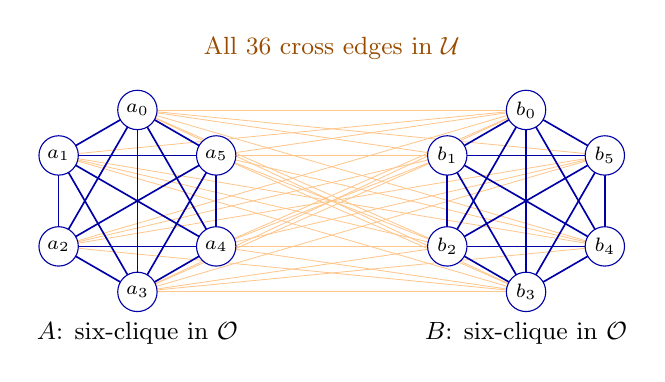
\begin{tikzpicture}[scale=1.05,
 dot/.style={circle,draw=blue!65!black,fill=white,inner sep=0pt,
 minimum size=5mm,font=\scriptsize}]
\foreach \i in {0,...,5} {
 \coordinate (a\i) at ({-2.35+1.1*cos(90+60*\i)},{1.1*sin(90+60*\i)});
 \coordinate (b\i) at ({2.35+1.1*cos(90+60*\i)},{1.1*sin(90+60*\i)});
}
\foreach \i in {0,...,5} \foreach \j in {0,...,5}
 \draw[orange!45,line width=.3pt] (a\i)--(b\j);
\foreach \i in {0,...,5} \foreach \j in {0,...,5} {
 \ifnum\i<\j
  \draw[blue!65!black,line width=.6pt] (a\i)--(a\j);
  \draw[blue!65!black,line width=.6pt] (b\i)--(b\j);
 \fi
}
\foreach \i in {0,...,5} {
 \node[dot] at (a\i) {$a_{\i}$};
 \node[dot] at (b\i) {$b_{\i}$};
}
\node[font=\small] at (-2.35,-1.6) {$A$: six-clique in $\mathcal O$};
\node[font=\small] at (2.35,-1.6) {$B$: six-clique in $\mathcal O$};
\node[font=\small,text=orange!60!black] at (0,1.85) {All $36$ cross edges in $\mathcal U$};
\end{tikzpicture}
\caption{Two further mutually unbiased bases would require twelve
distinct vector-ball labels: six pairwise orthogonality-compatible labels
in each set, with every cross pair unbiasedness-compatible. The graphs
retain all necessary edges. A completed search excluding this pattern
therefore excludes the two bases throughout the phase ball.}
\label{fig:two-cliques}
\end{figure}


\begin{lemma}[Complete graph search]
\label{exclude:graph-search}
The mode-$1$ search of \texttt{graph::exist}, started with both pools
equal to the full vertex set and first-clique target size six, returns
false only if \eqref{exclude:graph-configuration} is impossible.
A work-cap exhaustion never gives a negative certificate.
\end{lemma}
\begin{proof}
First consider \texttt{clique} on a candidate set $P$ and target size
$m$.  For $m=0$ it succeeds, and for $m=1$ it tests nonemptiness.
For $m\ge2$, it repeatedly selects the least remaining vertex $i$,
removes it from $P$, and searches $P\cap N_{\mathcal O}(i)$ for an
$(m-1)$-clique.  For $m=2$ that search is just nonemptiness.
Every clique has a unique least vertex, so this enumerates every
possibility.  Terminating when fewer than $m$ candidates remain is
also exact.

Now suppose that $A,B$ satisfy \eqref{exclude:graph-configuration}.
Interchange their names if necessary so that
$a=\min(A\cup B)$ belongs to $A$.
At the root, \texttt{exist} tries possible least vertices of the
first clique in increasing order.  It deletes each tried root vertex
from both its local first pool and its second pool.  Thus when $a$
is selected, every required remaining vertex in $A\cup B$ is still
available.  This root deletion imposes only the chosen convention
that the minimum of the union lies in the first clique.  It is
performed only when the remaining first-clique target is six,
and therefore not in any recursive call.

After an increasing prefix $S\subseteq A$ has been selected, with
$1\le|S|\le5$, the recursive first pool is the set of vertices larger
than $\max S$ that are $\mathcal O$-adjacent to every vertex of $S$.
The second pool is the set of vertices larger than $a$ that are
$\mathcal U$-adjacent to every vertex of $S$.
Selecting the next vertex $i$ intersects the remaining first pool
with $N_{\mathcal O}(i)$ and the second pool with
$N_{\mathcal U}(i)$.  In the branch selecting the next member of $A$,
these pools still contain the required remaining members of $A$ and
all of $B$, respectively.
The lack of $\mathcal U$ self-loops also removes every selected
first-clique vertex from the second pool.

A first-pool cardinality check cannot reject a pool containing the
needed remaining vertices.  A second-pool cardinality check cannot
reject a pool containing $B$.
The mode-$1$ prune runs the exact auxiliary six-clique test on the
second pool: it too must succeed if $B$ is present, and later
intersections can only shrink that pool.  On selection of the sixth
first-clique vertex, an auxiliary six-clique test of the resulting
second pool is exactly the remaining requirement.
Hence a complete branch survives for every configuration
\eqref{exclude:graph-configuration}.

Finally, all recursive tests interpret exhaustion of the work budget
as possibility and set a persistent give-up flag.  The public
\texttt{candidate} result is the logical disjunction of its search
result and this flag.  A negative result therefore requires both
an exhausted combinatorial search with no configuration and an unset
give-up flag; hitting the cap cannot certify exclusion.
\end{proof}

The graph has at most $2048$ vertices and is represented by $32$
unsigned 64-bit words per adjacency set.  Only valid vertex indices
are inserted, all unused bits are zero, and intersections and
cardinalities are exact integer operations.  A least-set-bit operation
is called only on a nonempty set.  Thus the finite-set operations in
the preceding proof are the operations performed by the code.
The specified search uses mode $1$ and a cap of $5{,}000{,}000$ steps.

\begin{proposition}[Local exclusion certificate]
\label{exclude:local-certificate}
Assume the root certificate
\eqref{exclude:root-data}--\eqref{exclude:root-decomposition} and the
arithmetic guarantees of Section~\ref{sec:rounding}.
If Stage C returns a negative result for the Record, then no exact
Hadamard $e(P+\delta)$ in its closed horizontal radius-$r$ ball can
be extended, together with the coordinate basis, by two further
mutually unbiased orthonormal bases.
\end{proposition}
\begin{proof}
Every additional vector belongs to a bin at the initial resolution.
The necessary tests retain a bin path containing it at all four
resolutions.  If the retained set becomes empty, no such vector
exists.  Otherwise a successful clustering covers all retained bins
by closed balls.  Two additional bases would give twelve distinct
ball labels with every required edge retained, hence a configuration
\eqref{exclude:graph-configuration}.  A completed negative graph
search excludes that configuration by
Lemma~\ref{exclude:graph-search}.
Overflow, clustering failure, a surviving graph possibility, and
work-cap exhaustion are all unresolved outcomes and are never
reported as negative.  These are exactly the two successful negative
paths of \texttt{negative}: an empty completed bin layer, or a
completed negative graph search.
\end{proof}

\subsection{Conservative arithmetic and invocation}
\label{exclude:implementation}

We finish by specifying the outward replacements and comparison margins
that connect the necessary inequalities to the implemented certificate.
Their arithmetic justification is in Sections~\ref{round:single}
and~\ref{round:joint}.

For a bin the source forms its halfwidth with a $10^{-12}$ increase,
then increases each of $X_M,L_M,I_M$ by a further $10^{-12}$ after
the indicated multiplication.  The stored tangent and normal bounds
are formed as
\[
 \widehat r_H=\sqrt{1+\omega}\,r+10^{-9},\qquad
 \widehat n=n_0+\iota r+\Gamma r^2+10^{-9}.
\]
The upper scalar squared-magnitude threshold in
\eqref{exclude:direct-tests} is increased by $2\cdot10^{-7}$,
and its lower threshold, when $\tau<1$, is decreased by that amount.
The combined squared-distance threshold, the right side of
\eqref{exclude:scalar-linear}, and the right side of
\eqref{exclude:bin-support} each receive a $2\cdot10^{-7}$ comparison
allowance.

For a pair, the radius sum is increased by $10^{-10}$.
The distance tests \eqref{exclude:edge-distance} permit a further
$2\cdot10^{-7}$ on that radius.  Both edge residual bounds
$E_{\mathcal O}$ and $E_{\mathcal U}$ are increased by $2\cdot10^{-8}$;
the direct comparisons \eqref{exclude:orth-support} and
\eqref{exclude:unbiased-support} receive another $2\cdot10^{-7}$.
The right side of the joint comparison
\eqref{exclude:joint-inequality} receives $3\cdot10^{-7}$.
Cluster assignment radii include the $10^{-9}$ allowance already
described in Lemma~\ref{exclude:cluster-cover}.

The bounds $|P_{ij}|\le4$ and $|v_j|\le2$ keep all trigonometric
arguments used here within the guarded range of \texttt{expair}.
The proof of Section~\ref{sec:rounding} includes the errors in these
arguments, in $q,S,c,J,B$, in the short weighted sums and norms, and in
the positive support expressions.  Inexact solution of the proposal
systems supplies no separate assumption.

For clarity, the invocation parameters used for this certificate are
\texttt{12 4 1 .042 1 1 5000000}: initial resolution $12$, four bin
layers, one proposed bin direction, clustering parameter $.042$,
one proposed joint direction, graph mode $1$, and the stated graph
work cap.  The two Lloyd iterations are the fixed default.
The conclusion of Proposition~\ref{exclude:local-certificate} is
conditional on a completed negative result for the individual Record;
no collection of unexecuted tests is itself such a result.
